\documentclass{article}
\usepackage{amsfonts} 
\usepackage{amsmath} 
\usepackage{graphicx}
\usepackage[ruled,vlined]{algorithm2e}
\usepackage{xcolor}

\DeclareMathOperator*{\argmin}{argmin} % no space, limits underneath in displays
\DeclareMathOperator*{\argmax}{argmax} % no space, limits underneath in displays

\begin{document}

\section{Basic Idea}
The basic idea is to seperate the gridgraph into a set of pairs
$\mathbb{S}~=~\{(A_i, B_i)~|~i~\in~\mathbb{N}\}$
such that $\forall (A, B) \in \mathbb{S}: A, B \subseteq V \land A \cap B = \emptyset$
and for each pair $u, v \in V$ there exists a pair $(A, B) \in \mathbb{S}$ such that $a \in A \land b \in B$ or
$b \in A \land a \in B$.
Furthermore, given a pair $(A, B) \in \mathbb{S}$, it should be easy to calculate optimal distances for paths from nodes $u \in A$
to $v \in B$ and the other way arround.
Since for every pair of nodes $u, v \in V$ there exists a pair $(A, B) \in \mathbb{S}$ with $a \in A \land b \in B$ or
$b \in A \land a \in B$, the calculation of the optimal distance between $u$ and $v$ boils down to finding such a pair $(A, B) \in\mathbb{S}$
and then reporting the optimal distance.
\quad\\



This means the challenge of finding the optimal distances for a gridgraph fast breaks down into two subchallenges:
\begin{itemize}
\item \textbf{Preprocessing:} calculating set $\mathbb{S}$ with the given properties and a way of reporting the optimal distances between nodes of $A$ and $B$.
\item \textbf{Query:} for a given pair $u, v \in V$, finding a set $a \in A \land b \in B$ or $b \in A \land a \in B$ must be fast.
\end{itemize}

In the following different approaches for the preprocessing and query phase are presented.

\section{Separation}
The idea of node separations comes from the well-separated pair decomposition, which organizes a given point set $P$
such that all of $\binom{P}{2}$ distances between points are clustered in into a linear amount of clusters,
and that all distances in each cluster are roughly the same.

In order to achieve this a QuadTree is build for the point set $P$ and then algorithm~\ref{alg:SeparateWSPD}
with the QuadTree root as input is called to calculate the well separation.

\begin{figure}[ht!]
  \begin{algorithm}[H]
    \KwData{QuadTree Nodes $X, Y$}
    \KwResult{Cluster Set $\mathbb{S}$}
    \If{$X = Y$}{
      \Return{$\emptyset$}
    }
    \If{$size(X) < size(Y)$}{
      \Return{$SeparateWSPD(Y, X)$}
    }
    \If{$areWellSeparated(X, Y)$}{
      \Return{$\{(X, Y)\}$}
    }

    \Return{$\bigcup_{C \in child(X)} SeparateWSPD(C, Y)$}
    \caption{SeparateWSPD}
    \label{alg:SeparateWSPD}
  \end{algorithm}
\end{figure}

Notice how the $areWellSeparated(X, Y)$ function can be used specify when two clusters are well-separated.
In order to be useable for shortest path distance queries, three different $areWellSeparated$ function could be used.

\begin{enumerate}
\item \textbf{Trivial Separation:} $X$ and $Y$ are well separated \\
  $\iff \forall u \in X: \forall v \in Y: d_{opt}(u, v) = |u_1 - v_1| + |u_2 - v_2|$\\
  where $d_{opt}(u, v)$ is the optimal distance between $u$ and $v$.
\item \textbf{Portal Separation:} $X$ and $Y$ are well separated \\
  $\iff \exists u_{portal} \in X: \exists v_{portal} \in Y: \forall u \in X: \forall v \in Y: u_{portal}~\in~\pi(u, v)~\land~v_{portal}~\in~\pi(u, v)$\\
  where $\pi(u, v)$ is one optimal path from $u$ to $v$.\\
  This means that there exists a portal node in $X$ and a portal node in $Y$ which is part of all shortest paths from $X$ to $Y$.

\item \textbf{Barrier Separation:}\\
  \textcolor{red}{not implemented\\}
  $X$ and $Y$ are well separated \\
  $\iff \exists b \in V: \forall u \in X: \forall v \in Y: b~\in~\pi(u, v)$\\
  which means that there exists a barrier node $b \in V$ that every shortest path from $X$ to $Y$ goes throught this node.

\end{enumerate}

\subsection{Trivial Separation}
To check wether two quadtree nodes $X$ and $Y$ are trivial separatable is easily achievable with algorithm~\ref{alg:TrivialSeparationCheck}.
An example of a trivial separation in a gridgraph can be seen in figure~\ref{pic:TrivialSeparation}.

\begin{figure}[ht!]
  \centering
  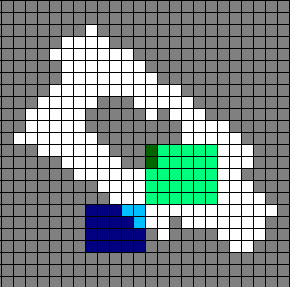
\includegraphics[width=0.33\textwidth]{TrivialSeparation.png}
  \caption{trivial separation example}
  \label{pic:TrivialSeparation}
\end{figure}


\begin{figure}[ht!]
  \begin{algorithm}[H]
    \KwData{QuadTree Nodes $X, Y$}
    \KwResult{$Boolean$}
    \For{$x \in X$}{
      \For{$y \in Y$}{
        $dist \longleftarrow d(x, y)$;\\
        $trivialDist \longleftarrow |x_1 - y_1| + |x_2 - y_2|$;\\

        \If{$dist \ne trivialDist$}{
          \Return{$FALSE$}
        }
      }
    }
    \Return{$TRUE$}
    \caption{TrivialSeparationCheck}
    \label{alg:TrivialSeparationCheck}
  \end{algorithm}
\end{figure}

\subsubsection*{Query}
When $X$ and $Y$ which are trivial separated are known for a given query $(x, y)$ the answer to the query is $|x_1 - y_1| + |x_2 - y_2|$.

\subsubsection{Lazy Path Reconstruction}
\textcolor{red}{not implemented\\}

\subsection{Portal Separation}
To calculate if two quadtree nodes $X$ and $Y$ are protal separatabel the two portals need to be found first.
The two portal candidates of a two quadtree nodes are the two nodes $x \in X$ and $y \in Y$ with the minimal distance.

\begin{equation}
  (x_{portal}, y_{portal}) = \argmin_{(x, y) \in X \times Y} d_{opt}(x, y)
\end{equation}

With those two portal candidates algorithm~\ref{alg:PortalSeparation} can find out if two quadtree nodes are portal separated.

\begin{figure}[ht!]
  \begin{algorithm}[H]
    \KwData{QuadTree Nodes $X, Y$, Portal Candidates $x_{portal}, y_{portal}$}
    \KwResult{$Boolean$}
    \For{$x \in X$}{
      \For{$y \in Y$}{
        \If{$d_{opt}(x, y) \ne d_{opt}(x, x_{potal}) + d_{opt}(x_{portal}, y_{portal}) + d_{opt}(y, y_{potal})$}{
          \Return{$FALSE$}
        }
      }
    }
    \Return{$TRUE$}
    \caption{PortalSeparationCheck}
    \label{alg:PortalSeparation}
  \end{algorithm}
\end{figure}

An example of a portal separation in a gridgraph can be seen in figure~\ref{pic:PortalSeparation}.

\begin{figure}[ht!]
  \centering
  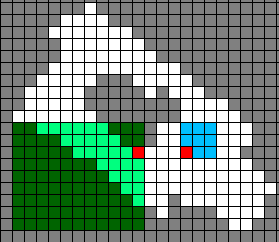
\includegraphics[width=0.33\textwidth]{PortalSeparation.png}
  \caption{portal separation example}
  \label{pic:PortalSeparation}
\end{figure}


\subsubsection{Query}
In order to answer a query, for each portal separated quadtree node pair $(X, Y)$, the two portals $x_{portal}, y_{portal}$ and the distance
between them $d_{opt}(x_{portal}, y_{portal})$ needs to be stored.
With those things stored the algorithm~\ref{alg:PortalQuery} can be used to answer queries.

\begin{figure}[ht!]
  \begin{algorithm}[H]
    \KwData{QuadTree Nodes $X, Y$, Query Nodes $u \in X, v \in Y$, Portal Candidates $x_{portal}, y_{portal}$}
    \KwResult{$d_{opt}(u, v)$}
    \If{$u = x_{portal} \land v = y_{portal}$}{
      \Return{$d_{opt}(x_{portal}, y_{portal})$}
    }

    \If{$u = x_{portal}$}{
      \Return{$d_{opt}(x_{portal}, y_{portal}) + PortalQuery(y_{portal}, v)$}
    }

    \If{$v = y_{portal}$}{
      \Return{$PortalQuery(x, x_{portal}) + d_{opt}(x_{portal}, y_{portal})$}
    }

    \Return{$PortalQuery(x, x_{portal}) + d_{opt}(x_{portal}, y_{portal}) + PortalQuery(y_{portal}, v)$}

    \caption{PortalQuery}
    \label{alg:PortalQuery}
  \end{algorithm}
\end{figure}

\subsection{Separation Optimization}
\subsubsection{Avoiding Neigbours}
Since the distance from a node to its neigbour is easly calculatable in a gridgraph, all separations $(X, Y)$ with $|X| = |Y| = 1$
and $\forall x \in X: \forall y \in Y: x~and~y~are~neigbours$  can be omitted.

\subsubsection{Separation Weight Optimization}
The algorithm~\ref{alg:SeparateWSPD} does only compare quadtree nodes with a heigh difference of at most 1.
While this leads to optimal and unambiguous separations for points, it does not for nodes in a gridgraph.
To further optimize the separations a comparison between different separations is needed.
in the following, the weight of a separation $(X, Y)$ is defined as:

\begin{equation*}
  weight((X, Y)) = |\{x~|~x \in X~\land~x~is~walkable\}| \cdot |\{y~|~y \in Y~\land~y~is~walkable\}|
\end{equation*}

Intuitively the weight of a separation is the number of node pairs for which it is able to answer optimal distance queries.


Furthermore domination of one separation of another is defined as:
\begin{equation*}
  (X, Y) \preceq (A, B) = (A \subseteq X \land B \subseteq Y) \lor (B \subseteq X \land A \subseteq Y)
\end{equation*}

If one separation is dominated by another separation it can be omitted, since all node pair queries can also be answered by the
dominating one.\\

\quad\\

Separations can be seen as blue edges between the well-separated nodes in the quadtree. Such a set of blue nodes can be optimized by
trying to push the blue edges higher in the quadtree. Since the original algorithm only connects two quadtree nodes with a high difference of at most
1, often such blue edges can be pushed higher in the quadtree. In order to do this the two nodes of a separation are used as a lower bound,
which means the blue edge will not be pushed below the nodes of quadtree.
As an upper bound the first quadtree node which both nodes of the separation are a subset of is used.
Let $parent(A, B)$ be the set of nodes in the quadtree of which are $A$ and $B$ subsets, and $parent(A)$ all nodes which are node $A$ is a subset of.
Then in order to push the the blue edge higher, algorithm~\ref{alg:pushBlueEdge} can be used to push a blue edge higher.
When a new separation with a better weight is found, it can be possible that one of the known separations is dominated by the newly found separation.
If that is the case, the dominated separation can be deleted. This leads to the optimization algorithm~\ref{alg:OptSeparations}

\begin{figure}[ht!]
  \begin{algorithm}[H]
    \KwData{Separation ($X, Y$)}
    \KwResult{Separation ($X_{new}, Y_{new}$)}
    $bestWeight~\longleftarrow~weight(X, Y)$;\\
    $bestSeparation~\longleftarrow~(X, Y)$;\\
    \For{$x \in parent(X) \setminus parent(X, Y)$}{
      \For{$y \in parent(Y) \setminus parent(X, Y)$}{
        \If{$weight(x, y) < bestWeight$}{
          continue;
        }

        \If{$isWellSeparated(x, y)$}{
          $bestWeight~\longleftarrow~weight(x, y)$;\\
          $bestSeparation~\longleftarrow~(x, y)$;\\
        }

      }
    }

    \Return{$bestSeparation$}

    \caption{pushBlueEdge}
    \label{alg:pushBlueEdge}
  \end{algorithm}
\end{figure}

\begin{figure}[ht!]
  \begin{algorithm}[H]
    \KwData{Set of Separations $S$}
    \KwResult{Optimized Separations $S_{new}$}
    \For{$(A, B) \in S$}{
      $(A_{new}, B_{new}) \longleftarrow pushBlueEdge((A, B))$
      $S \longleftarrow S \setminus {(x, y)~|~(x, y) \in~S \land (x, y) \preceq (A_{new}, B_{new})}$
    }

    \Return{$S$}

    \caption{optimizeSeparations}
    \label{alg:OptSeparations}
  \end{algorithm}
\end{figure}

\subsection{Distance Query}
When given two nodes $u, v \in V$ it should be possible to get the shortest path distance as fast as possible.
To do this, for every node $u$ all the separations $(A, B)$ are stored where $u \in A \lor u \in B$.
Using this, it is trivial to access all the separations of a node which can be used to answer distance queries.
In order to do this the separation for which holds $u \in A \land v \in B$ or $v \in A \land u \in B$ needs to be found.

\subsubsection{Linear Scan}
When given all separations of node $u$, the separation which can answer the query $u, v$ can be found by searching through all the
given separations.

\subsubsection{Z Order Curve}
\textcolor{red}{not implemented\\}
When the gridgraph has a hight and a width of $2^n$ for any $n \in \mathbb{N}$ a Z-Curve
can be used to map from a 2D point $v$ to a number in $\mathbb{N}$ such that the prefixes of the number in binary format can be used to
identify the quadtree nodes which the node $v$ is a member of.

\subsubsection{Quadtree Prefix}
\textcolor{red}{not implemented\\}
Since not all all the gridgraphs have a width and a hight of $2^n$ for any $n \in \mathbb{N}$,
the quadtree can be used to assign numbers from $n \in \mathbb{N}$ for every node $v \in V$, such that the prefixes of the numbers identify the quadtree nodes a gridgraph node is a member of.
These prefixes can be used to build a descision tree for each set of separations such that every separation for any node pair $u, v$ can be found in $\mathcal{O}(\log{}n)$.
Since only 64-bit numbers are being used, the decision tree can only be that high and the search can be considered $\mathcal{O}(1)$


\section{Node Patches}
Node selections are set of nodes $(A, B)$ such that:
\begin{equation*}
  \exists x \in V: \forall u \in A: \forall v \in B: x \in \pi(u, v)
\end{equation*}

To find such sets, the path between two random nodes $(a_0, b_0)$ is considered and then a node in the middle of the path is used as the barrier node.
The sets $\{a_0\}$ and $\{b_0\}$ can then be used to grow sets of nodes. In an alternating way neigbours of nodes in set $A$ and $B$ are looked at and then
checked if they fullfill the property that all shortest paths from the node to the other set of nodes can go over the barrier node $x$.
If that is the case the node is added to the set. The random start nodes can be choosen from a set containing all $\binom{V}{2}$ nodes, and node patches should be searched until for all node pairs $u, v \in V$ there exists a node patch which can answer the distance query of nodes $u, v$.
Figure~\ref{pic:NodePatch} shows such a node patch of two sets.

\begin{figure}[ht!]
  \centering
  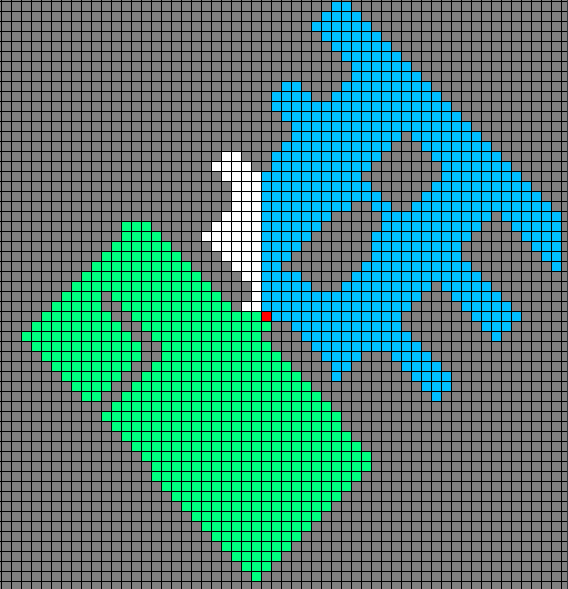
\includegraphics[width=0.33\textwidth]{NodePatch.png}
  \caption{node patch example}
  \label{pic:NodePatch}
\end{figure}

\subsection{Query}
Each node patch stores its nodes $(A, B)$ and the barrier node $x$.
For each node $n$ all node patches $(A, B)$ where $n \in A \lor n \in B$ are stored sorted.
Finding a node patch which can be used to answer a query $u, v \in V$ can be done in like it is done for HubLabels.
When the node patch $(A, B)$ with ${u \in A \land v \in B \lor v \in A \land u \in B}$ is found the query routine can be called
recursivly for nodes $u, x$ and $x, v$ where $x$ is the barrier node of the node patch $(A, B)$. This query routine can be seen in Algorithm~\ref{alg:queryNodePatch}.

\begin{figure}[ht!]
  \begin{algorithm}[H]
    \KwData{Node Patche $(A, B, x)$, Nodes $u, v$}
    \KwResult{$d_{opt}(u, v)$}

    \If{$u \in neig(v)$}{
      \Return{1}
    }

    \Return{$queryNodePatch(u, x) + queryNodePatch(x, v)$}

    \caption{queryNodePatch}
    \label{alg:queryNodePatch}
  \end{algorithm}
\end{figure}

\subsection{Node Patch Optimization}
\textcolor{red}{not implemented\\}
Since nodes have a common subsets of associated node patches $(A, B)$ subsets of all node patches can be stored in buckets which then are stored by the nodes, instead of lists of node patches.
In order to find optimal buckets $B \subseteq \mathcal{P}(S)$ of node patches for a set of separations $S$,
a set of nodes with associated separations ${N = \{(n, S_n)| n \in V, S_n \subseteq S\}}$, the follwowing musst be assured:
\begin{equation*}
  \forall (n, S_n) \in N: \exists B_n \in B: \forall s \in S_n: \exists b \in B_n: s \in b
\end{equation*}

To get a best possible result for the distance query structure $|B|$ and \linebreak
${\forall (n, S_n) \in N: |B_n|}$ musst be minimal, where $B_n$ are the buckets node $n$ stores.


\end{document}
